% Vector figures for pages 1--2. Requires tikz, xcolor, and \ifanswers.
% The main document defines answerred. All macros take no arguments.
\usetikzlibrary{decorations.pathreplacing}
\providecommand{\FFAns}[1]{\ifanswers\textcolor{answerred}{$#1$}\else\phantom{$#1$}\fi}
\tikzset{ffbox/.style={draw,line width=.45pt,minimum width=.82cm,minimum height=.40cm,inner sep=1.5pt,font=\small},
  ffop/.style={circle,draw,line width=.45pt,minimum size=.29cm,inner sep=0pt,font=\small},
  fflink/.style={line width=.45pt},
  ffbrace/.style={decorate,decoration={brace,amplitude=3pt},line width=.4pt}}

\newcommand{\FigLines}{%
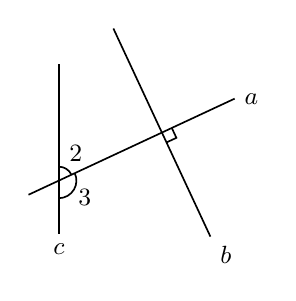
\begin{tikzpicture}[x=.77cm,y=.77cm,line width=.6pt,font=\small]
  \coordinate (O) at (2.2,1.42);
  \draw (0,.394)--(3.4,1.979) node[right]{$a$};
  \draw (1.4,3.136)--(3,-.296) node[below right]{$b$};
  \draw (.5,-.25)--(.5,2.55);
  \node[below] at (.5,-.25){$c$};
  % The square is exactly aligned with a and b (25-degree and -65-degree rays).
  \draw (2.3631,1.4961)--(2.4392,1.3330)--(2.2761,1.2569);
  \draw (.5,.6271) ++(25:.23) arc[start angle=25,end angle=90,radius=.23];
  \draw (.5,.6271) ++(-90:.29) arc[start angle=-90,end angle=25,radius=.29];
  \node at (.78,1.08){2};
  \node at (.93,.35){3};
\end{tikzpicture}}

\newcommand{\FigRoutes}{%
\begin{tikzpicture}[x=.88cm,y=.88cm,line width=.55pt,font=\small]
  \draw (0,2.10)--(4,2.10) (0,2.65)--(4,2.65);
  \node at (2,2.375){五一大街};
  \coordinate (H) at (2,0);
  \draw (H)..controls (1.40,.10) and (1.65,.55)..(1.05,.65)
    ..controls (.18,.8) and (.50,1.45)..(.15,2.10);
  \draw (H)--(2,2.10);
  \draw (H)--(2.75,2.10);
  \draw (H)..controls (3.65,.65) and (3.9,.85)..(3.85,2.10);
  \draw (2,1.91)--(2.19,1.91)--(2.19,2.10);
  \fill (H) circle[radius=1.5pt];
  \node[below] at (H){李芳家};
  \node at (.96,.42){$A$};
  \node[left] at (1.98,1.13){$B$};
  \node[right] at (2.46,1.07){$C$};
  \node[right] at (3.67,1.03){$D$};
\end{tikzpicture}}

\newcommand{\FigReceipt}{%
\begin{tikzpicture}[x=1cm,y=1cm,font=\small]
  \draw[line width=.55pt] (0,0) rectangle (3.65,1.72);
  \node[anchor=west] at (.15,1.42){单价：58元/件};
  \node[anchor=west] at (.15,1.04){数量：};
  \ifanswers
    \node[anchor=west,text=answerred] at (1.22,1.04){17};
  \else
    \fill[gray!35] (1.23,.89) rectangle (1.80,1.19);
  \fi
  \node[anchor=west] at (1.86,1.04){件};
  \node[anchor=west] at (.15,.66){付款金额：1000元};
  \node[anchor=west] at (.15,.28){找零：14元};
\end{tikzpicture}}

\newcommand{\FigTreeA}{%
\begin{tikzpicture}[x=.82cm,y=.71cm]
  \node[ffbox] (a) at (2.4,3.2){\FFAns{14}};
  \node[ffop] at (3.15,3.2){\FFAns{-}};
  \node[ffbox] (b) at (3.9,3.2){\FFAns{12}};
  \node[ffbox] (c) at (3.15,2.2){\FFAns{2}};
  \node[ffbox] (d) at (1.65,2.2){\FFAns{15}};
  \node[ffop] at (2.4,2.2){\FFAns{\times}};
  \node[ffbox] (e) at (2.4,1.2){\FFAns{30}};
  \node[ffbox] (f) at (.9,1.2){\FFAns{990}};
  \node[ffop] at (1.65,1.2){\FFAns{-}};
  \node[ffbox] (g) at (1.65,.2){\FFAns{960}};
  \draw[fflink] (a.south)--(c.north) (b.south)--(c.north)
    (c.south)--(e.north) (d.south)--(e.north)
    (e.south)--(g.north) (f.south)--(g.north);
\end{tikzpicture}}

\newcommand{\FigMultiplication}{%
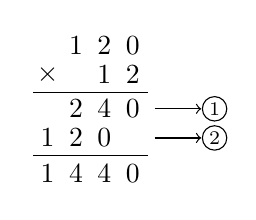
\begin{tikzpicture}[x=1cm,y=1cm,font=\normalsize]
  % Four fixed columns guarantee correct positional alignment.
  \node at (.36,1.82){$1$}; \node at (.72,1.82){$2$}; \node at (1.08,1.82){$0$};
  \node at (0,1.45){$\times$}; \node at (.72,1.45){$1$}; \node at (1.08,1.45){$2$};
  \draw[line width=.55pt] (-.18,1.23)--(1.28,1.23);
  \node at (.36,1.02){$2$}; \node at (.72,1.02){$4$}; \node at (1.08,1.02){$0$};
  \node at (0,.65){$1$}; \node at (.36,.65){$2$}; \node at (.72,.65){$0$};
  \draw[line width=.55pt] (-.18,.43)--(1.28,.43);
  \node at (0,.20){$1$}; \node at (.36,.20){$4$}; \node at (.72,.20){$4$}; \node at (1.08,.20){$0$};
  \draw[->,line width=.45pt] (1.36,1.02)--(1.95,1.02);
  \node[circle,draw,inner sep=1pt,font=\scriptsize] at (2.12,1.02){1};
  \draw[->,line width=.45pt] (1.36,.65)--(1.95,.65);
  \node[circle,draw,inner sep=1pt,font=\scriptsize] at (2.12,.65){2};
\end{tikzpicture}}

\newcommand{\FigChainOne}{%
\begin{tikzpicture}[x=.84cm,y=.70cm]
  \node[ffbox] (a) at (1.8,3.2){$52$};
  \node at (2.6,3.2){$+$};
  \node[ffbox] (b) at (3.4,3.2){$29$};
  \node[ffbox] (c) at (2.6,2.2){\FFAns{81}};
  \node[ffbox] (d) at (1,2.2){$26$};
  \node at (1.8,2.2){$\times$};
  \node[ffbox] (e) at (1.8,1.2){\FFAns{2106}};
  \node at (2.6,1.2){$-$};
  \node[ffbox] (f) at (3.4,1.2){$128$};
  \node[ffbox] (g) at (2.6,.2){\FFAns{1978}};
  \draw[fflink] (a.south)--(c.north) (b.south)--(c.north)
    (c.south)--(e.north) (d.south)--(e.north)
    (e.south)--(g.north) (f.south)--(g.north);
\end{tikzpicture}}

\newcommand{\FigChainTwo}{%
\begin{tikzpicture}[x=.84cm,y=.70cm]
  \node[ffbox] (a) at (1,3.2){$212$};
  \node at (1.8,3.2){$+$};
  \node[ffbox] (b) at (2.6,3.2){$460$};
  \node[ffbox] (c) at (1.8,2.2){\FFAns{672}};
  \node at (2.6,2.2){$\div$};
  \node[ffbox] (d) at (3.4,2.2){$24$};
  \node[ffbox] (e) at (2.6,1.2){\FFAns{28}};
  \node[ffbox] (f) at (1,1.2){$20$};
  \node at (1.8,1.2){$\times$};
  \node[ffbox] (g) at (1.8,.2){\FFAns{560}};
  \draw[fflink] (a.south)--(c.north) (b.south)--(c.north)
    (c.south)--(e.north) (d.south)--(e.north)
    (e.south)--(g.north) (f.south)--(g.north);
\end{tikzpicture}}

\newcommand{\FigRelations}{%
\begin{tikzpicture}[x=1cm,y=1cm,font=\small,line width=.5pt]
  \foreach \x/\lab/\ffouter/\ffinner in {0/A/相交/互相垂直,3.9/B/相交/互相平行,7.8/C/互相平行/互相垂直}{
    \begin{scope}[xshift=\x cm]
      \node at (.05,.94){\lab.};
      \draw (1.85,.93) ellipse[x radius=1.50,y radius=.70];
      \node at (1.85,1.28){\ffouter};
      \draw (1.85,.70) ellipse[x radius=1.02,y radius=.27];
      \node at (1.85,.70){\ffinner};
    \end{scope}
  }
\end{tikzpicture}}

\newcommand{\FigBars}{%
\begin{tikzpicture}[x=1cm,y=1cm,font=\footnotesize,line width=.5pt]
  % A: known whole and one known part.
  \begin{scope}
    \node at (0,.71){A.};
    \draw (.35,.61) rectangle (3.00,.81);
    \draw (1.02,.61)--(1.02,.81);
    \draw[ffbrace] (.35,.94)--(1.02,.94) node[midway,above=3pt]{16元};
    \draw[ffbrace] (1.02,.94)--(3.00,.94) node[midway,above=3pt]{?元};
    \draw[ffbrace] (3.00,.45)--(.35,.45) node[midway,below=3pt]{50元};
  \end{scope}
  % B: sum of three different prices.
  \begin{scope}[xshift=3.8cm]
    \node at (0,.71){B.};
    \draw (.35,.61) rectangle (3.00,.81);
    \draw (1.00,.61)--(1.00,.81) (1.80,.61)--(1.80,.81);
    \draw[ffbrace] (.35,.94)--(1.00,.94) node[midway,above=3pt,xshift=-2pt]{10元};
    \draw[ffbrace] (1.00,.94)--(1.80,.94) node[midway,above=3pt,xshift=2pt]{14元};
    \draw[ffbrace] (1.80,.94)--(3.00,.94) node[midway,above=3pt]{26元};
    \draw[ffbrace] (3.00,.45)--(.35,.45) node[midway,below=3pt]{?元};
  \end{scope}
  % C: 48 yuan plus 16 yuan; the common part is three equal units.
  \begin{scope}[xshift=7.6cm]
    \node at (0,.71){C.};
    \draw (.35,1.00) rectangle (2.33,1.20);
    \draw (1.01,1.00)--(1.01,1.20) (1.67,1.00)--(1.67,1.20);
    \draw[ffbrace] (.35,1.33)--(2.33,1.33) node[midway,above=3pt]{48元};
    \draw (.35,.45) rectangle (2.99,.65);
    \draw (1.01,.45)--(1.01,.65) (1.67,.45)--(1.67,.65) (2.33,.45)--(2.33,1.20);
    \draw[ffbrace] (2.33,.78)--(2.99,.78) node[midway,above=3pt]{16元};
    \draw[ffbrace] (2.99,.29)--(.35,.29) node[midway,below=3pt]{?元};
  \end{scope}
  % D: five equal portions. Unit price is 130 yuan.
  \begin{scope}[xshift=11.4cm]
    \node at (0,.71){D.};
    \draw (.35,.61) rectangle (3.00,.81);
    \foreach \x in {.88,1.41,1.94,2.47}{\draw (\x,.61)--(\x,.81);}
    \draw[ffbrace] (.35,.94)--(.88,.94) node[midway,above=3pt]{130元};
    \draw[ffbrace] (3.00,.45)--(.35,.45) node[midway,below=3pt]{?元};
  \end{scope}
\end{tikzpicture}}

\newcommand{\FigConstructOne}{%
\begin{tikzpicture}[x=1cm,y=1cm,line width=.7pt,font=\small]
\coordinate (A) at (0,2.8);\coordinate (B) at (5.7,2.0);\coordinate (C) at (0,.2);\coordinate (D) at (5.7,1.0);\coordinate (P) at (2.6,1.55);
\draw (A)--(B);\draw (C)--(D);
\node[left] at(A){$A$};\node[right] at(B){$B$};\node[left]at(C){$C$};\node[right]at(D){$D$};\fill(P)circle(1.2pt);\node[above right]at(P){$P$};
\ifanswers
\draw[answerred] (-.2,1.943) node[left]{$l$}--(5.9,1.087);
\coordinate (H) at ($(C)!(P)!(D)$);
\draw[answerred] ($(P)!-1.3!(H)$) node[above right]{$m$}--($(P)!2.0!(H)$);
\draw[answerred] ($(H)!.22cm!(D)$)--++(98:.22)--($(H)!.22cm!(P)$);
\node[answerred,below]at(2.85,-.65){$l\parallel AB,\quad m\perp CD$};
\fi
\end{tikzpicture}}
\newcommand{\FigConstructTwo}{%
\begin{tikzpicture}[x=1cm,y=1cm,line width=.7pt,font=\small]
\coordinate(B)at(0,0);\coordinate(C)at(20:5.2);\coordinate(H)at(20:2.6);\coordinate(A)at($(H)+(110:2)$);
\draw(A)--(B)--(C)--cycle;
\node[above left]at(A){$A$};\node[below left]at(B){$B$};\node[right]at(C){$C$};
\ifanswers
\draw[answerred] ($(A)+(110:.5)$)--($(H)+(290:.5)$);
\draw[answerred] ($(A)+(200:2.8)$)--($(A)+(20:3.6)$) node[right]{$l$};
\draw[answerred] ($(H)+(20:.22)$)--++(110:.22)--($(H)+(110:.22)$);
\node[answerred,below right]at(H){$H$};
\path(A)--(H) node[midway,right,answerred]{2厘米};
\fi
\end{tikzpicture}}
\newcommand{\FigKnotTree}{%
\begin{tikzpicture}[x=1cm,y=1cm,font=\small,box/.style={draw,minimum width=3.4cm,minimum height=.65cm,inner sep=2pt},op/.style={draw,circle,minimum size=.55cm,inner sep=0pt}]
\node[box] (top) at(0,0){可以装多少盒？};
\node[box] (a) at(-2.5,-1.0){\Ans{合格个数：688}};\node[op]at(0,-1){\Ans{$\div$}};\node[box](b)at(2.5,-1){\Ans{每盒个数：8}};
\draw(top.south)--(a.north);\draw(top.south)--(b.north);
\node[box](c)at(-3.6,-2){\Ans{总个数：720}};\node[op]at(-1.5,-2){\Ans{$-$}};\node[box](d)at(.6,-2){\Ans{不合格个数：32}};
\draw(a.south)--(c.north);\draw(a.south)--(d.north);
\node[box](e)at(-4.7,-3){\Ans{每批个数：45}};\node[op]at(-2.6,-3){\Ans{$\times$}};\node[box](f)at(-.5,-3){\Ans{批数：16}};
\draw(c.south)--(e.north);\draw(c.south)--(f.north);
\end{tikzpicture}}
\newcommand{\FigTunnel}{%
\begin{tikzpicture}[x=1cm,y=1cm,font=\small,line width=.7pt]
\draw (0,0)--(12,0);\foreach\x in {0,1.36,2.72,4.08,5.44,7.08,8.72,10.36,12}{\draw (\x,-.12)--(\x,.12);}
\draw[->] (0,-.45)--(5.25,-.45);\draw[<-] (5.65,-.45)--(12,-.45);
\node at(2.72,-.85){开拓者队：每月350米，4个月};\node at(8.72,-.85){先锋队：每月420米，4个月};
\draw[decorate,decoration={brace,amplitude=5pt}] (0,.35)--(12,.35) node[midway,above=7pt]{2号线路全长？米};
\ifanswers\node[answerred,above]at(2.72,.1){1400米};\node[answerred,above]at(8.72,.1){1680米};\fi
\end{tikzpicture}}

\begin{document}
\Title
\Sect{一、填空题（每空1分，共25分）}
\Q{1}{$4\times\square+85\div5=77$，这道算式中，$\square$里应填（\Ans{15}\hspace{8mm}）。}
\Sol{先算除法：$85\div5=17$，再倒推：$77-17=60$，$60\div4=15$。检验：$4\times15+85\div5=60+17=77$。}
\Q{2}{小马虎在计算$(600-\square)\div25+94$时，漏看了小括号，算出的结果是678。他在检查时发现了这个错误，又重新计算。这道题的正确结果是（\Ans{102}\hspace{8mm}）。}
\Sol{错算为$600-\square\div25+94=678$，所以$\square\div25=600+94-678=16$，$\square=16\times25=400$。正确算式：
\[\begin{aligned}(600-400)\div25+94&=200\div25+94\\&=8+94\\&=102.\end{aligned}\]}
\Q{3}{如图，直线$a$与直线$b$互相（\Ans{垂直}\hspace{5mm}），图中共有（\Ans{4}\hspace{5mm}）个直角，直线$b$与直线$c$（\Ans{相交}\hspace{5mm}）。}
\begin{center}\FigLines\end{center}
\Sol{两条直线互相垂直形成4个直角。$b$与$c$不是平行线，延长后会相交。}
\Q{4}{如图所示，李芳家通往五一大街有4条路线，长度分别是900米、1千米、1800米和2千米，可以判断B路线的长度是（\Ans{900米}\hspace{6mm}）。}
\begin{center}\FigRoutes\end{center}
\Sol{B是从李芳家到五一大街的垂线段，最短。统一单位后为900米、1000米、1800米、2000米，所以B长900米。}
\ifanswers\newpage\fi
\Q{5}{西安是“一带一路”的起点。一位外国商人在西安采购了一批相同的服装。如图，采购小票不小心被弄脏了，付款金额1000元，找零14元。$1000-14$计算的是（\Ans{购买服装的总价}\hspace{8mm}），$(1000-14)\div58$计算的是（\Ans{购买服装的数量}\hspace{8mm}）。}
\begin{center}\FigReceipt\end{center}
\Sol{付款减找零得到总价：$1000-14=986$（元）；总价除以单价得到数量：$986\div58=17$（件）。此处填所求数量的名称。}
\Q{6}{一架农用无人机喷洒农药，飞行速度为每分钟200米，喷幅（喷洒宽度）为4米。它加满一箱药可以连续飞行8分钟。加一次药最多能完成（\Ans{6400}\hspace{9mm}）平方米农田的喷洒。}
\Sol{方法一，先求飞行距离：\[\begin{aligned}200\times8\times4&=1600\times4\\&=6400\text{（平方米）}.\end{aligned}\]方法二，先求每分钟喷洒面积：\[\begin{aligned}200\times4\times8&=800\times8\\&=6400\text{（平方米）}.\end{aligned}\]}
\ifanswers\else\newpage\fi
\Q{7}{把$754-28\times9\div3$的运算顺序改为先求差和商，最后求积，那么原来的算式要变为（\Ans{$(754-28)\times(9\div3)$}\hspace{10mm}）。}
\Sol{把求差、求商的两部分分别放进小括号：$(754-28)\times(9\div3)$。只写$(754-28)\times9\div3$时，最后一步仍是除法，不符合要求。}
\Q{8}{计算$990-[15\times(14-12)]$时，应先算（\Ans{减}\hspace{5mm}）法，再算（\Ans{乘}\hspace{5mm}）法，最后算（\Ans{减}\hspace{5mm}）法。把计算过程写在下图中。}
\begin{center}\FigTreeA\end{center}
\Sol{$990-[15\times(14-12)]=990-[15\times2]=990-30=960$。先小括号，再中括号，最后括号外。}
\Q{9}{列车平均每小时行驶120千米，行驶了12小时。根据下面竖式填空。}
\begin{minipage}[c]{0.70\linewidth}
（1）解决这个问题，用到的数量关系是\par（\Ans{速度$\times$时间$=$路程}\hspace{10mm}）。\par
（2）箭头\textcircled{\scriptsize 1}所指的表示（\Ans{2}\hspace{5mm}）小时行驶的路程。\par
（3）箭头\textcircled{\scriptsize 2}所指表示（\Ans{10}\hspace{5mm}）小时行驶（\Ans{1200}\hspace{5mm}）千米。
\end{minipage}\hfill\begin{minipage}[c]{0.27\linewidth}\centering\FigMultiplication\end{minipage}
\Sol{个位2表示2小时，$120\times2=240$。十位1表示10小时，$120\times10=1200$。第二部分积“120”左移一位，实际表示1200。}
\ifanswers\newpage\fi
\Q{10}{先填空，再列综合算式。（每题2分）}
\begin{minipage}[t]{0.48\linewidth}\centering （1）\par\FigChainOne\par 综合算式：\par\ifanswers{\color{answerred}$26\times(52+29)-128=1978$}\else\blank[7.7cm]\fi\end{minipage}\hfill
\begin{minipage}[t]{0.48\linewidth}\centering （2）\par\FigChainTwo\par 综合算式：\par\ifanswers{\color{answerred}$20\times[(212+460)\div24]=560$}\else\blank[7.7cm]\fi\end{minipage}
\Sol{\begin{align*}26\times(52+29)-128&=26\times81-128=2106-128=1978,\\20\times[(212+460)\div24]&=20\times[672\div24]=20\times28=560.\end{align*}}
\ifanswers\else\vfill\newpage\fi
\Sect{二、选择题（每题2分，共16分）}
\Q{1}{“（\quad）”是17世纪荷兰数学家吉拉尔首先使用的。在这之前，曾经有人用括线“$\overline{\quad\quad}$”表示算式中先算的部分。算式“$429-\overline{29+15}\times6$”的运算顺序是什么？（\Ans{C}\hspace{5mm}）}
\begin{tabular}{@{}ll@{}}A. 先算减法，再算加法，最后算乘法 & B. 先算乘法，再算加法，最后算减法\\C. 先算加法，再算乘法，最后算减法 & D. 先算乘法，再算减法，最后算加法\end{tabular}
\Sol{横括线与小括号作用相同：$429-(29+15)\times6$。先算$29+15=44$，再算$44\times6=264$，最后算$429-264=165$，选C。}
\Q{2}{下面运算顺序相同的一组算式是（\Ans{A}\hspace{5mm}）。}
\begin{center}\begin{tabular}{@{}c@{\qquad}c@{\qquad}c@{\qquad}c@{}}A. $\begin{cases}32+19-13\\13\times25\div5\end{cases}$& B. $\begin{cases}98-56\div8\\(91-67)\times4\end{cases}$ & C. $\begin{cases}49\div7\times13\\98-81\div9\end{cases}$ & D. $\begin{cases}24\times(63-24)\\15\times7-28\end{cases}$\end{tabular}\end{center}
\Sol{A组两道算式都从左往右算。B、C、D各组的两道算式，先后计算的位置不同，选A。}
\Q{3}{下列算式中，去掉小括号，运算顺序不变的是（\Ans{A}\hspace{5mm}）。}
\begin{center}A. $(53\times15)+28\div4$\qquad B. $85\div5+(94-89)$\qquad C. $(36+27)\div9\times3$\end{center}
\Sol{A中乘法原本就先于加法，小括号可以去掉。B去掉后不再先算$94-89$；C去掉后不再先算$36+27$。}
\ifanswers\newpage\fi
\Q{4}{把一张长方形纸对折，再对折，然后展开，折痕间的关系是（\Ans{C}\hspace{5mm}）。}
\begin{tabular}{@{}ll@{}}A. 一定互相平行 & B. 一定互相垂直\\C. 可能互相垂直，也可能互相平行 & D. 既不互相垂直，也不互相平行\end{tabular}
\Sol{通常沿长方形对称轴对折：两次沿同一方向折，展开可有平行折痕；换一个方向折，展开可有垂直折痕。因此选C。题目按小学常规对折语境理解。}
\Q{5}{下面关系图正确的是（\Ans{A}\hspace{5mm}）。}
\begin{center}\FigRelations\end{center}
\Sol{互相垂直是相交的一种特殊情况，因此“互相垂直”应包含在“相交”之内，选A。}
\Q{6}{一列火车长500米，以每分钟900米的速度经过一座大桥，从车头进桥到车尾离桥用了3分钟。求桥长的正确列式是（\Ans{B}\hspace{5mm}）。}
\begin{center}A. $900\times3+500$\qquad B. $900\times3-500$\qquad C. $(900+500)\times3$\end{center}
\Sol{车头走过的路程是“桥长$+$车长”。因此桥长为$900\times3-500=2700-500=2200$（米），选B。}
\Q{7}{下面四幅图中的问题，能用数量关系“单价$\times$数量$=$总价”解决的是（\Ans{D}\hspace{5mm}）。}
\begin{center}\FigBars\end{center}
\Sol{D表示每份130元，共5份：$130\times5=650$（元）。A通常求$50-16$，B求$10+14+26$，C通常求$48+16$。按题目意图，D直接表示单价$\times$数量，选D；C也可先推每份16元，再用$16\times4$求解，因此原题“能用”的措辞不够严密。}
\Q{8}{在计算$27+27\times27-27\div27$时，最后一步求的是（\Ans{D}\hspace{5mm}）。}
\begin{center}A. 积\hspace{2cm} B. 和\hspace{2cm} C. 商\hspace{2cm} D. 差\end{center}
\Sol{$27+27\times27-27\div27=27+729-1=756-1=755$。最后一步是减法，求差，选D。}
\newpage
\Sect{三、计算（原卷标“共25分”）}
\textbf{1. 直接写得数。}（原卷标“每题1分，共7分”）\par
{\footnotesize\color{notegrey}校勘：原图实际有8道口算题，全部保留；原卷本节分值与题数不一致。}\par
\renewcommand{\arraystretch}{2.0}
\begin{tabular}{@{}p{.47\linewidth}p{.47\linewidth}@{}}
（1）$5\times24=\Ans{120}$ &（2）$330\div3=\Ans{110}$\\
（3）$24\times30=\Ans{720}$ &（4）$(35-20)\times20\div4=\Ans{75}$\\
（5）$360\div12=\Ans{30}$ &（6）$480\div8=\Ans{60}$\\
（7）$720\div18=\Ans{40}$ &（8）$39\times8\div39\times8=\Ans{64}$
\end{tabular}\renewcommand{\arraystretch}{1}\par
\Sol{口算提示：（1）$5\times20+5\times4=100+20=120$；（2）$33\div3=11$，所以$330\div3=110$；（3）$24\times3=72$，再乘10；（4）先括号，再从左往右：$15\times20\div4=300\div4=75$。\par
（5）$12\times30=360$；（6）$8\times60=480$；（7）$18\times40=720$；（8）乘除同级，从左往右：$39\times8\div39\times8=312\div39\times8=8\times8=64$，不能把后面的$39\times8$整体当作除数。}
\vspace{4pt}\textbf{2. 脱式计算。}（每题3分，共18分）\par
\begin{minipage}[t]{.48\linewidth}
（1）$240\div80+14\times2$
\Sol{\[\begin{aligned}&240\div80+14\times2\\&=3+28\\&=31\end{aligned}\]}
\Work{2.1cm}
\end{minipage}\hfill\begin{minipage}[t]{.48\linewidth}
（2）$108-(83+360\div60)$
\Sol{\[\begin{aligned}&108-(83+360\div60)\\&=108-(83+6)\\&=108-89\\&=19\end{aligned}\]}
\Work{2.1cm}
\end{minipage}\par
\begin{minipage}[t]{.48\linewidth}
（3）$(432+48)\div(375-345)$
\Sol{\[\begin{aligned}&(432+48)\div(375-345)\\&=480\div30\\&=16\end{aligned}\]}
\Work{2.1cm}
\end{minipage}\hfill\begin{minipage}[t]{.48\linewidth}
（4）$(480+120)\div(12\times5)$
\Sol{\[\begin{aligned}&(480+120)\div(12\times5)\\&=600\div60\\&=10\end{aligned}\]}
\Work{2.1cm}
\end{minipage}\par
\begin{minipage}[t]{.48\linewidth}
（5）$957\div[(316-294)\div2]$
\Sol{\[\begin{aligned}&957\div[(316-294)\div2]\\&=957\div(22\div2)\\&=957\div11\\&=87\end{aligned}\]}
\Work{2.1cm}
\end{minipage}\hfill\begin{minipage}[t]{.48\linewidth}
（6）$46\times[(2022-1977)\div9]$
\Sol{\[\begin{aligned}&46\times[(2022-1977)\div9]\\&=46\times(45\div9)\\&=46\times5\\&=230\end{aligned}\]}
\Work{2.1cm}
\end{minipage}
\newpage
\Sect{四、作图题（共5分）}
\Q{1}{过点$P$分别画出直线$AB$的平行线和直线$CD$的垂线。}
\begin{center}\FigConstructOne\end{center}
\Sol{用直尺和三角板平移作出过$P$的直线$l$，使$l\parallel AB$；再过$P$作直线$m\perp CD$，在交点补直角符号。两条作出的线都要经过$P$，并向点的两侧延长。}
\Q{2}{画一画。\par（1）过$A$点作线段$BC$的垂线，并量出$A$点到直线$BC$的距离。\par（2）过$A$点作线段$BC$的平行线。}
\begin{center}\FigConstructTwo\end{center}
\ifanswers\else 距离：\blank[3cm]厘米。\par\fi
{\footnotesize\color{notegrey}本题图形重新按比例绘制；测量请按100\%原尺寸打印，不选“适应页面”。}
\Sol{过$A$作$AH\perp BC$，垂足为$H$。距离是垂线段$AH$的长度。本重排版按100\%原尺寸打印时，$AH$约为2厘米。再过$A$作$l\parallel BC$。照片无法可靠恢复原卷纸面的厘米长度，2厘米仅对应本重排图。}
\newpage
\Sect{五、解决问题（共29分）}
\Q{1}{手工艺坊制作了16批中国结，每批45个。质检时发现有32个不合格，剩下的每8个装一个礼品盒，可以装多少盒？（将分析过程补充完整）}
\begin{center}\FigKnotTree\end{center}
\Sol{方法一：先求合格的中国结个数，再求盒数。\[
\begin{aligned}(45\times16-32)\div8&=(720-32)\div8\\&=688\div8\\&=86\text{（盒）}.\end{aligned}\]
方法二：先求全部装盒数，再减去不合格个数相当的盒数。\[
\begin{aligned}45\times16\div8-32\div8&=720\div8-4\\&=90-4\\&=86\text{（盒）}.\end{aligned}\]
答：可以装86盒。}
\Work{2.6cm}
\ifanswers\newpage\fi
\Q{2}{建设美好新农村，富兴村绿化要购进一批树苗和花苗。}
\begin{center}\renewcommand{\arraystretch}{1.35}\begin{tabular}{|c|c|c|c|c|}\hline 品种 & 广玉兰 & 桂花 & 丁香 & 牡丹\\\hline 单价/元 &55& & $38^{\dagger}$&36\\\hline\end{tabular}\renewcommand{\arraystretch}{1}\end{center}
{\footnotesize\color{notegrey}$\dagger$ 照片中丁香单价暂辨认为38元，仍有可能为36元；本题按38元计算，答案版同时列出36元时的结果。}
\par（1）买了179棵丁香和79棵牡丹，购买丁香比牡丹多花多少元？
\Sol{方法一：分别求总价，再求差。\[
\begin{aligned}38\times179-36\times79&=6802-2844\\&=3958\text{（元）}.\end{aligned}\]
方法二：丁香多买了100棵；同为79棵的部分每棵又贵2元。\[
\begin{aligned}38\times(179-79)+(38-36)\times79&=38\times100+2\times79\\&=3800+158\\&=3958\text{（元）}.\end{aligned}\]
答：按丁香每棵38元计算，多花3958元。\par 若原表丁香实际为36元，则$36\times(179-79)=36\times100=3600$（元）。}
\Work{2.6cm}
\par（2）买了广玉兰和桂花各26棵，一共花了2600元，桂花的单价是多少元？
\Sol{方法一：每组各1棵，共26组。\[
\begin{aligned}2600\div26-55&=100-55\\&=45\text{（元）}.\end{aligned}\]
方法二：先扣去广玉兰费用，再求桂花单价。\[
\begin{aligned}(2600-55\times26)\div26&=(2600-1430)\div26\\&=1170\div26\\&=45\text{（元）}.\end{aligned}\]
答：桂花的单价是45元。}
\Work{2.2cm}
\newpage
\Q{3}{某地正在建设一条跨海高铁海底隧道，其中的2号线路由开拓者队、先锋队两个工程队从两端同时施工。开拓者队每月修350米，先锋队每月修420米，4个月完工。}
\par（1）2号线路长多少米？（先画图整理条件和问题，再列式解答）
\ifanswers\begin{center}\FigTunnel\end{center}\else\vspace{2.0cm}\fi
\Sol{方法一：先求两队每月合修的长度。\[
\begin{aligned}(350+420)\times4&=770\times4\\&=3080\text{（米）}.\end{aligned}\]
方法二：分别求两队4个月修的长度。\[
\begin{aligned}350\times4+420\times4&=1400+1680\\&=3080\text{（米）}.\end{aligned}\]
答：2号线路长3080米。}
\Work{1.4cm}
\par（2）完成时，开拓者队比先锋队少修多少米？
\Sol{方法一：先求每个月少修多少米。\[
\begin{aligned}(420-350)\times4&=70\times4\\&=280\text{（米）}.\end{aligned}\]
方法二：两队修的总长度相减。\[
\begin{aligned}420\times4-350\times4&=1680-1400\\&=280\text{（米）}.\end{aligned}\]
答：开拓者队比先锋队少修280米。}
\Work{1.4cm}
\ifanswers\newpage\fi
\Q{4}{军军周末去爬山，他上山时的速度为每小时800米，走完上山全程用了3小时；之后沿原路下山，只用了2小时。}
\par（1）军军上山的路程是多少米？
\Sol{上山路程$=$上山速度$\times$上山时间。\[800\times3=2400\text{（米）}.\]答：军军上山的路程是2400米。}
\Work{1.3cm}
\par（2）在整个上山和下山的往返过程中，军军平均每小时行多少米？
\Sol{往返总路程除以总时间。\[
\begin{aligned}800\times3\times2\div(3+2)&=2400\times2\div5\\&=4800\div5\\&=960\text{（米）}.\end{aligned}\]
答：军军平均每小时行960米。\par 也可列式$(2400+2400)\div(3+2)=4800\div5=960$（米），这是同一思路的另一种写法。\par 注意：上、下山所用时间不同，不能直接把两个速度相加后除以2。}
\Work{1.7cm}
\ifanswers\newpage\fi
\Sect{附加题}
\Q{1}{天天在计算$700-(320-\star\div4)$时，把括号里的运算顺序弄错了，先算了$320-\star$的差，这样得到的结果为690。这道题正确的结果是多少？}
\Sol{错算相当于$700-[(320-\star)\div4]=690$。从错误结果逆推：
\[700-690=10,\qquad10\times4=40,\qquad320-40=280.\]
所以$\star=280$。再按正确顺序计算：\[
\begin{aligned}700-(320-280\div4)&=700-(320-70)\\&=700-250\\&=450.\end{aligned}\]
答：这道题正确的结果是450。}
\Work{1.6cm}
\Q{2}{同学们去秋游，汽车以每小时42千米的速度行驶了3小时后，距目的地还有18千米。如果返回时用了4小时，那么返回时的平均速度是多少？}
\Sol{按返回沿原路的通常题意，返程路程等于去程全程。\[
\begin{aligned}(42\times3+18)\div4&=(126+18)\div4\\&=144\div4\\&=36\text{（千米/时）}.\end{aligned}\]
答：返回时的平均速度是每小时36千米。}
\Work{1.4cm}
\ifanswers
\vfill
\begingroup\footnotesize\color{notegrey}
\textbf{校勘说明}\par
1. 原卷第三大题口算列出8题，却标“每题1分，共7分”；本版保留所有题目，未擅自调整原分值。\par
2. 花苗表丁香单价暂读38元，照片低清，36元的可能性仍须原卷核实。两个分支的计算结果均已给出。\par
3. 作图题重新绘制，距离测量按本版100\%打印；不能从照片确定原卷厘米长度。\par
4. 隧道题“高铁”二字照片不清，也可能为“高速”；不影响数量条件和解答。选择题第1题的历史介绍依原题保留，未作为本版另行核实的史学结论。\par
5. 选择题第4题按小学常见的长方形对称轴对折理解；附加题第2题按沿原路返回理解。\par
\endgroup
\fi
\end{document}
